\documentclass[10pt]{article}
\usepackage[letterpaper,margin=1.6cm]{geometry}\usepackage{graphicx,booktabs,xcolor,amsmath,hyperref}
\definecolor{navy}{HTML}{102A43}\definecolor{teal}{HTML}{2A9D8F}\hypersetup{colorlinks=true,urlcolor=teal}\pagestyle{plain}\setlength{\parindent}{0pt}\setlength{\parskip}{5pt}
\begin{document}\begin{titlepage}\pagecolor{navy}\color{white}\raggedright\vspace*{1cm}{\Large DEEP LEARNING Y SISTEMAS INTELIGENTES\par}\vspace{1cm}{\Huge\bfseries Proyecto 1\\[.25cm]Monitoreo transaccional\par}\vspace{.7cm}{\LARGE Variables causales, boosting y validación temporal\par}\vfill{\Large Universidad del Valle de Guatemala\\Kevin Recinos · Grupo 1 · Sección 30\\Semestre II 2026\par}\vspace{1cm}{\Large Wilson Alejandro Calderón Argueta · 22018\\Pablo Daniel Barillas Moreno · 22193\par}\vfill\textbf{Nota:} el 15\% final es un benchmark histórico reutilizado, no test ciego.\end{titlepage}\nopagecolor
\section*{Resumen ejecutivo} Se analizaron 590,540 transacciones IEEE-CIS con prevalencia 3.50%. V2 preserva V1, amplía variables y audita ausencia, correlación, información mutua y redundancia. El ganador interno fue \textbf{LightGBM\_corr\_pruned}. En benchmark histórico, LightGBM alcanzó AP 0.4536 y el ensamble calibrado 0.4379. La decisión combina ranking, recall, costo y calibración.
\section{Datos y causalidad} Las tablas se unieron por TransactionID y ordenaron por TransactionDT. Ninguna de ambas se interpreta como predictor continuo. Los códigos de tarjeta/dirección/dispositivo son categorías o proxies. Para cada $t$, $x_t^{hist}=f(\{x_j:t_j<t\})$. Se calculan conteo y monto previos, razón de monto, tiempo anterior y actividad de 1/6/24/72 horas. El protocolo usa 70\% entrenamiento, 15\% validación y 15\% benchmark reutilizado; tres ventanas internas simulan reentrenamientos.

La clave tarjeta--dirección produce 42,946 entidades y una mediana de 2.0 transacciones. 87.7\% de los eventos pertenece a proxies con al menos ocho observaciones y 80.2\% a proxies con al menos dieciséis. Se compararon además tarjeta--dirección--correo y tarjeta--dispositivo--producto. Esta cobertura establece si una ventana secuencial nominal tiene antecedentes reales; una clave demasiado específica fragmenta y una demasiado amplia mezcla usuarios.

\section{Selección, correlación y PCA} Pearson captura linealidad, Spearman monotonía e información mutua dependencia no lineal; ninguna implica causalidad. Se excluyen constantes, alta ausencia e IDs. Pares con $|\rho_s|\ge 0.985$ se depuran por relevancia. Quedan 110 numéricas y 18 categóricas. PCA se ajusta por fold tras imputar/escalar solo numéricas elegibles. Explicar 95\% de varianza no garantiza separar fraude.

La selección se aprendió únicamente en el primer 55\% temporal. Esto impide que el patrón de ausencia o la distribución de un período posterior determine qué variable se conserva. Variables con baja asociación marginal no se eliminan automáticamente: pueden resultar informativas por interacción. El umbral alto de redundancia solo retira sustitutos casi monotónicos y registra para cada exclusión la variable retenida y su coeficiente.
\begin{figure}[h]\centering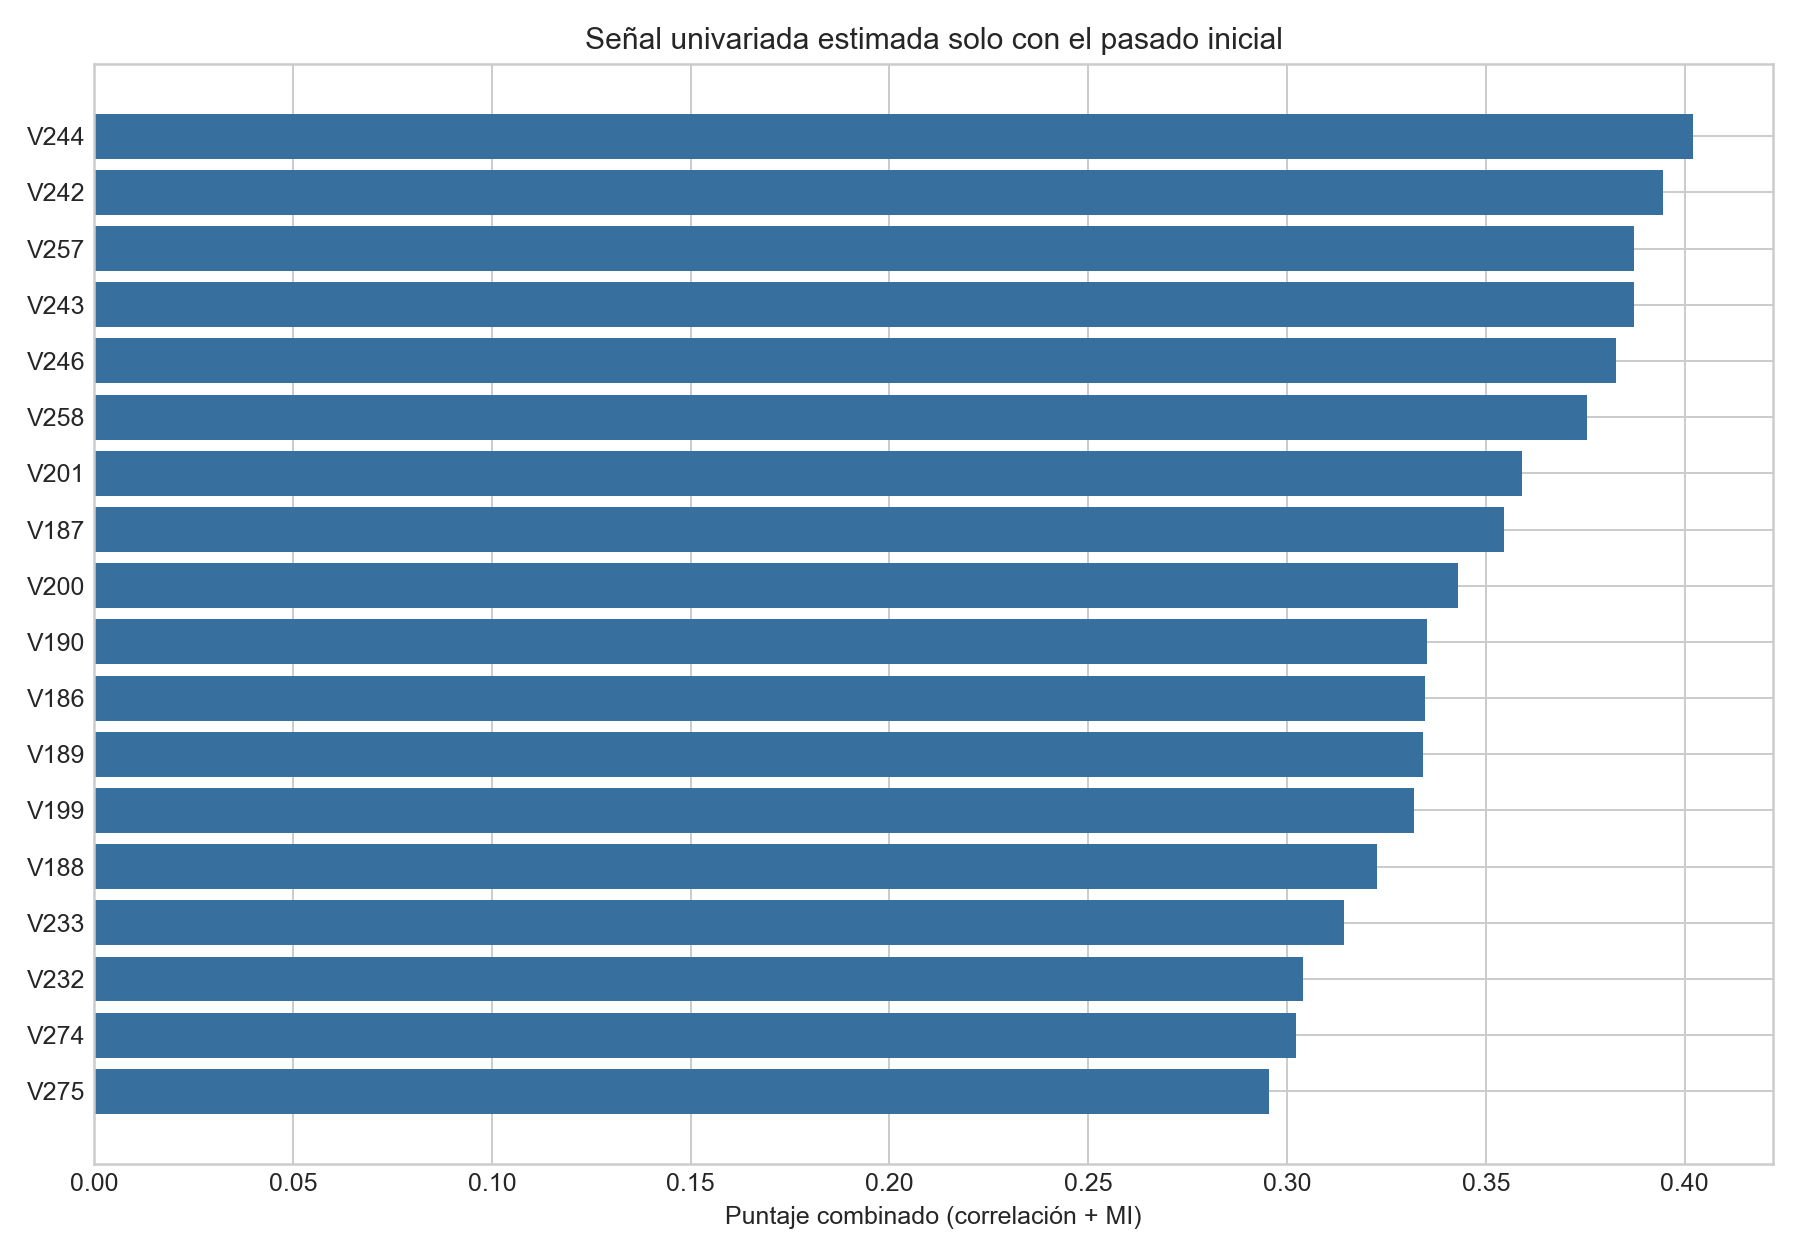
\includegraphics[width=.78\linewidth]{../../evidencia/figuras/v2/03_relevancia_variables.png}\caption{Señal estimada en el pasado inicial.}\end{figure}
\newpage
\section{Modelos y validación} LightGBM usa variables depuradas; CatBoost conserva categorías nativas con 240 iteraciones; LightGBM+PCA mide compresión. El ensamble logístico combina score tabular y agregados causales, y reserva el final de validación para calibración y umbral. No se denomina A+B-GRU porque no usa predicciones OOF GRU V2.

La media walk-forward fue 0.4727 para LightGBM depurado, 0.4580 para CatBoost y 0.4494 para PCA95. Sus tiempos medios fueron aproximadamente 24.8, 398.6 y 33.4 segundos, respectivamente. Por tanto, PCA redujo dimensionalidad pero perdió señal supervisada, y CatBoost no compensó su costo computacional bajo el presupuesto documentado. Esto no demuestra inferioridad universal de ambos enfoques; delimita su rendimiento bajo este protocolo.

La ablación de muestra obtuvo AP de validación 0.4661 con 180,000 filas, 0.4682 con 300,000 y 0.4664 con las 413,378 filas. La ventaja pequeña de 300k sobre el conjunto completo es compatible con deriva o menor utilidad de observaciones antiguas. Se mantiene el entrenamiento completo como modelo principal para representar toda la diversidad, pero el hallazgo se conserva como evidencia negativa.
\begin{figure}[h]\centering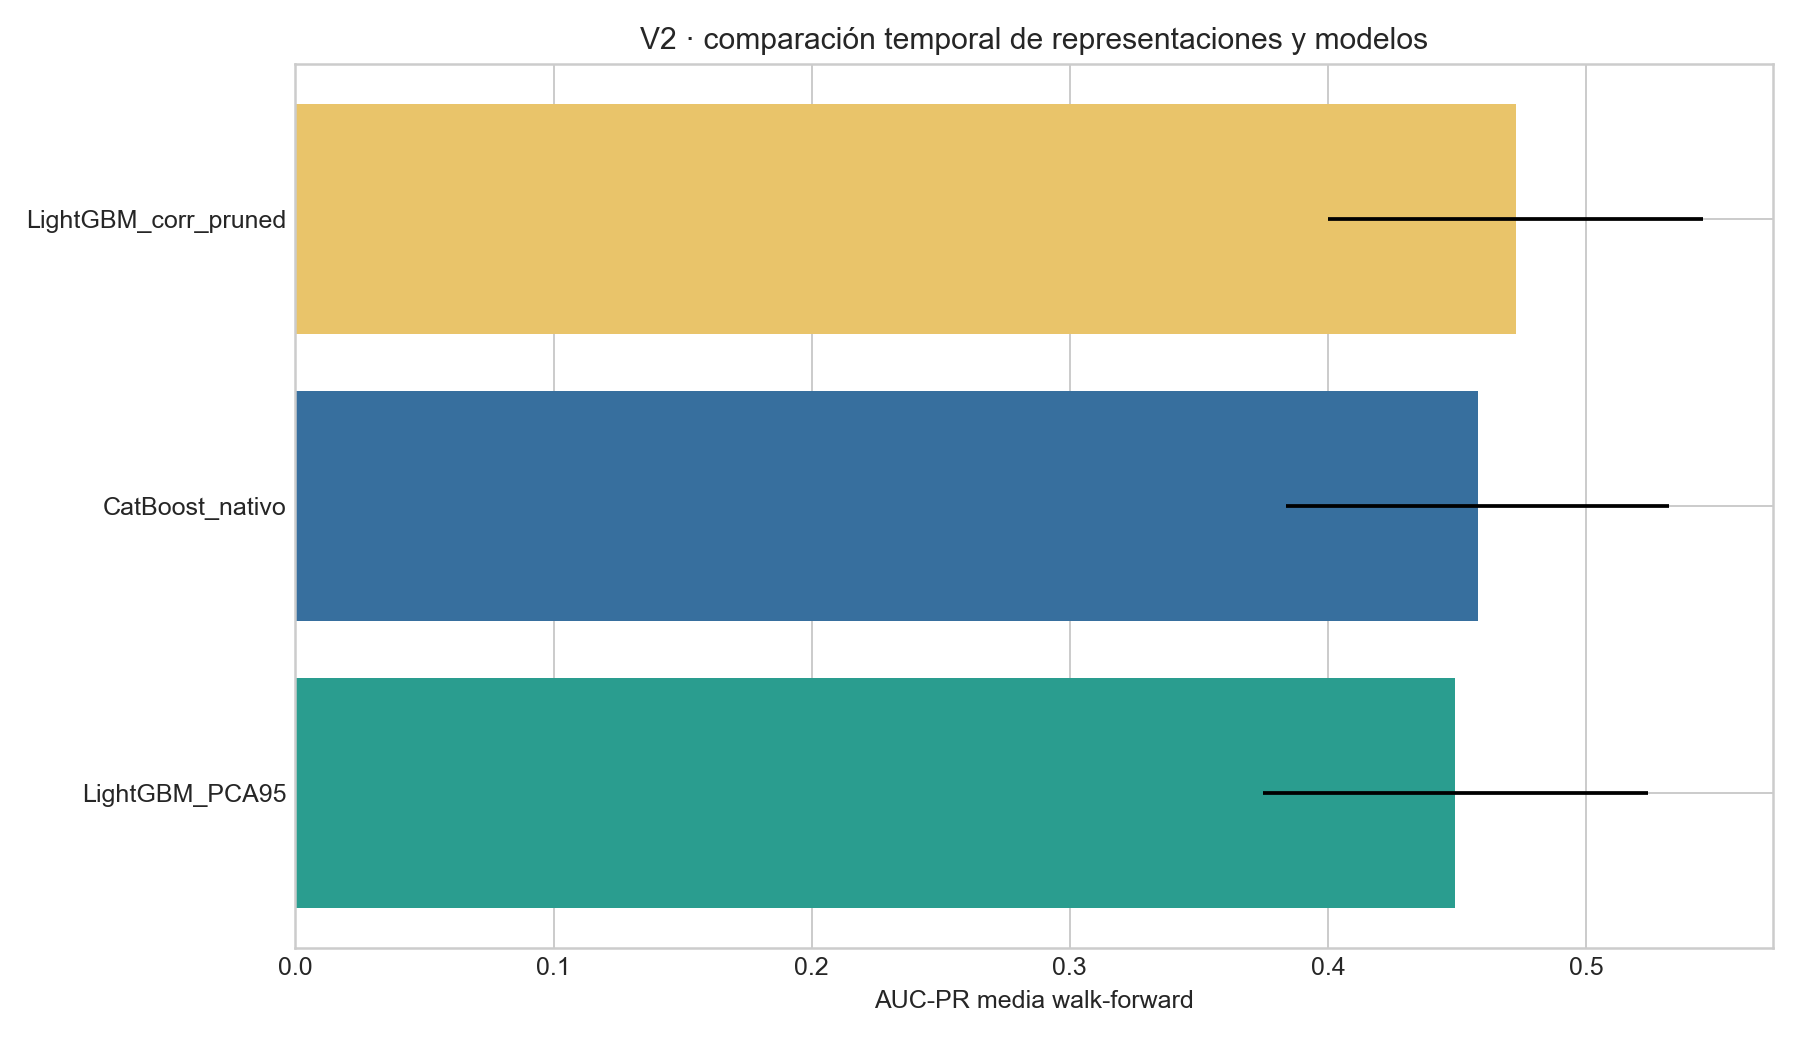
\includegraphics[width=.82\linewidth]{../../evidencia/figuras/v2/01_validacion_walk_forward.png}\caption{Comparación walk-forward.}\end{figure}
\newpage
\section{Resultados y economía}\begin{center}\begin{tabular}{lrrrrr}\toprule Modelo&AUC-PR&Precisión&Recall&F1&Costo\\\midrule LightGBM V2&0.454&0.149&0.703&0.246&Q6,078,120\\Ensamble&0.438&0.141&0.702&0.235&Q6,228,600\\\bottomrule\end{tabular}\end{center} El costo $4200FN+180FP$ hace que recall tenga gran peso. Mejor F1 no implica menor costo. Para LightGBM V2, el intervalo AP por bloques es [0.4113, 0.4918]. Precision@K/Recall@K traducen ranking a capacidad.

Frente a V1, LightGBM V2 aumenta AP de 0.4285 a 0.4536 y reduce el costo de Q6,193,620 a Q6,078,120. El recall baja de 0.7217 a 0.7029; la reducción de falsos positivos compensa económicamente bajo los costos fijados, pero un operador que privilegie fraude recuperado podría elegir otro umbral. La decisión debe presentarse con esta tensión, no solamente con la mejora de AP.

El ensamble tiene AP 0.4379 y costo Q6,228,600, peores que LightGBM. Se rechaza como candidato final y se conserva el resultado: agregar señales causales a un metamodelo no garantiza información incremental si el árbol ya explota esas variables.
\begin{figure}[h]\centering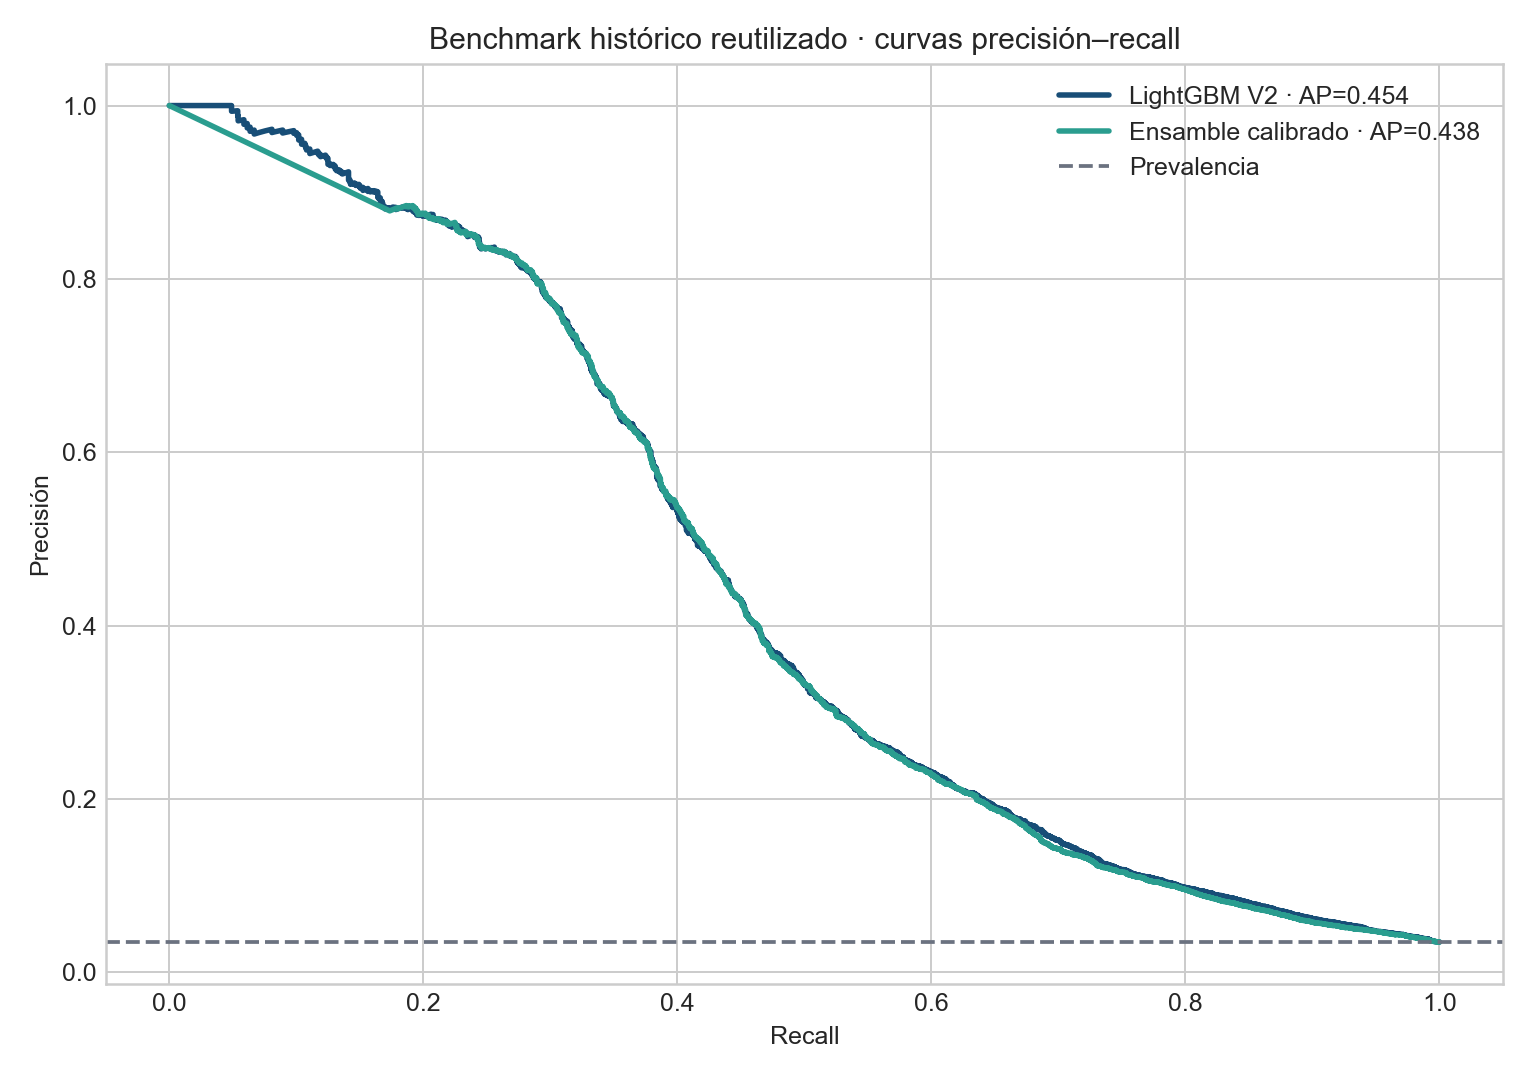
\includegraphics[width=.65\linewidth]{../../evidencia/figuras/v2/02_curvas_pr_v2.png}\end{figure}
\newpage
\section{Calibración, operación y errores} Brier y ECE evalúan calidad probabilística. Se reportan producto, dispositivo, monto, deriva, alertas/100k y falsos negativos. Calibrar no necesariamente altera AUC-PR, pero estabiliza decisiones de riesgo. Antes de producción: cohorte nueva, privacidad, explicabilidad, sesgo, seguridad, costos reales y monitoreo.

En validación, el Brier tabular fue 0.0236; el del ensamble calibrado, 0.0242. ECE pasó de 0.0015 a 0.0049. Estas cifras se interpretan junto con AP: una escala probabilística mejor no rescata un ranking inferior.

La tasa de alertas LightGBM es 16438 por 100,000 transacciones en el umbral económico. Se guardan Precision@K y Recall@K para capacidades de 0.1\%, 0.5\%, 1\% y 2\%, además de desglose por ProductCD, DeviceType y cuartil de monto. La operación debe vigilar cambios de prevalencia, ausencia, monto, costo y volumen, pues un umbral fijo puede degradarse aun sin cambios de arquitectura.
\begin{figure}[h]\centering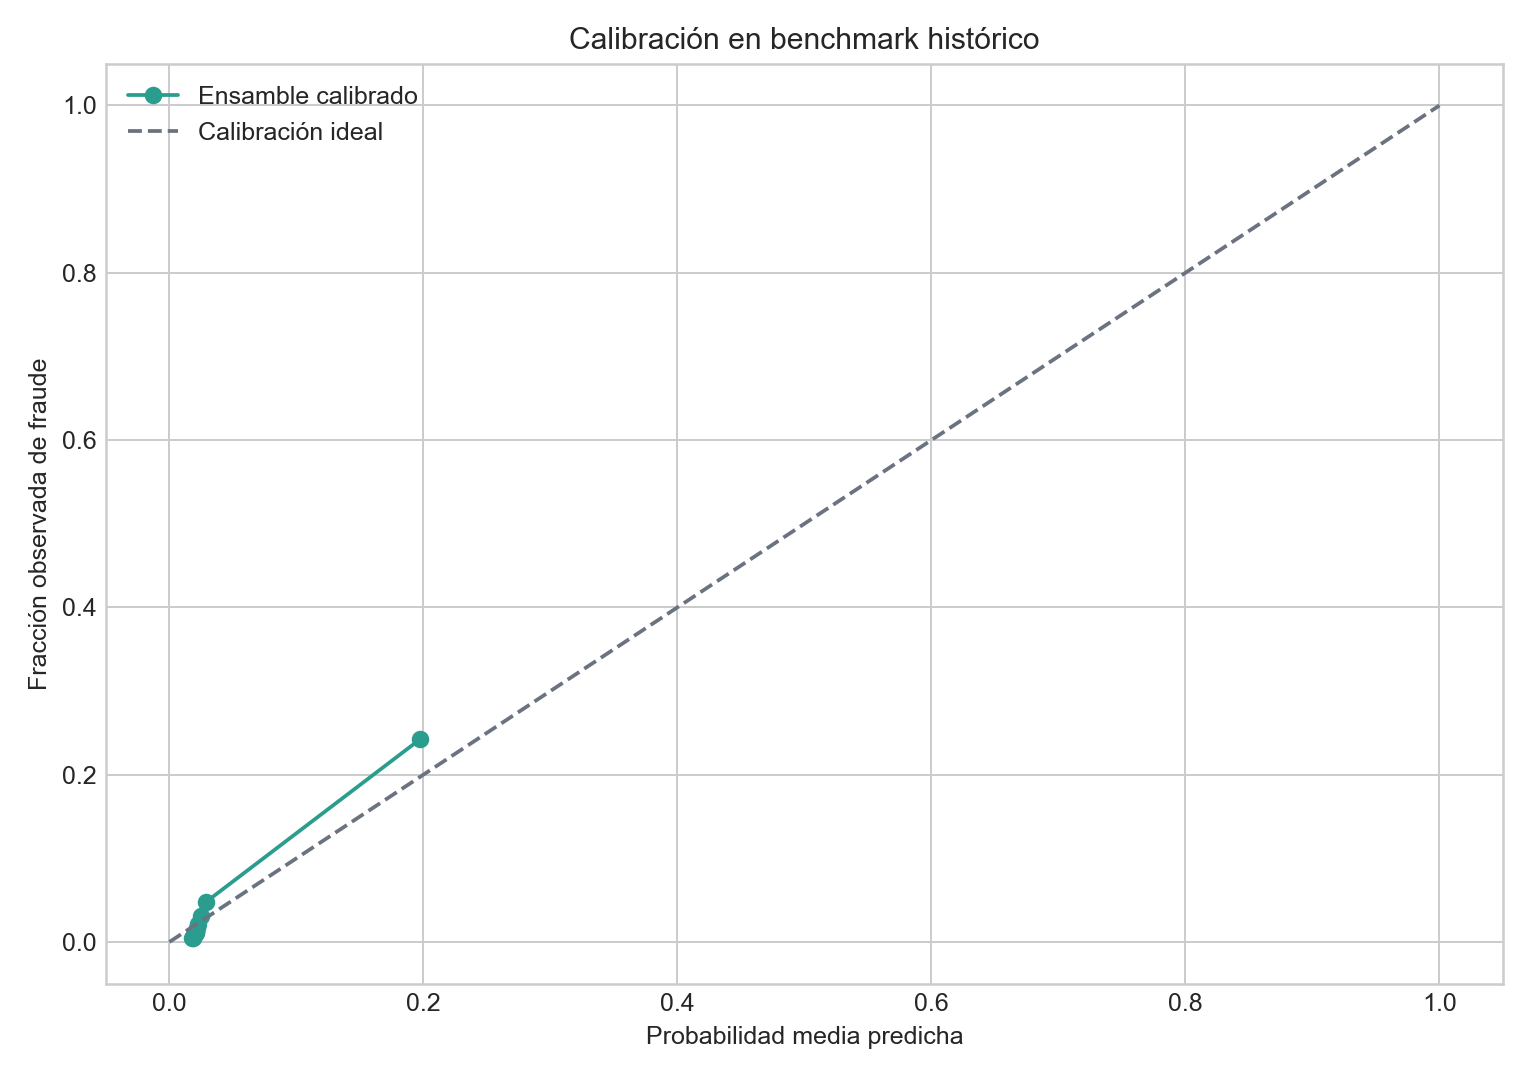
\includegraphics[width=.58\linewidth]{../../evidencia/figuras/v2/04_calibracion_v2.png}\end{figure}
\newpage
\section{Conclusión y hoja de ruta} La evidencia respalda mejorar datos antes de arquitectura. Correlación quita redundancia; PCA se acepta solo si gana temporalmente. V1 mostró orden débil. V3 debe usar cohorte nueva, OOF tabular+GRU, proxies alternativos, ventanas 3/8/16, Adam/AdamW, 6/12/20 épocas y focal loss; TCN/atención solo si la falsificación revela señal.

La recomendación actual es LightGBM V2 con representación depurada, acompañado por calibración y monitoreo, no el ensamble. Antes de congelar una siguiente versión se debe definir una cohorte nunca observada, producir predicciones out-of-fold de A y B, comparar stacking logístico, calibrar en un bloque separado y fijar el umbral antes de abrir el nuevo test. Una arquitectura secuencial mayor solo se justifica si permutar la historia produce una caída clara y repetible.
\section*{Limitaciones y ética} Benchmark reutilizado; identidad aproximada; anonimización; CatBoost acotado; costo académico. Uso exclusivo para priorizar revisión humana, no rechazo automático ni atribución de culpa.
\section*{Referencias}\small Ke, G., Meng, Q., Finley, T., Wang, T., Chen, W., Ma, W., Ye, Q., \& Liu, T.-Y. (2017). LightGBM: A highly efficient gradient boosting decision tree. \textit{NeurIPS, 30}.\\Prokhorenkova, L., Gusev, G., Vorobev, A., Dorogush, A. V., \& Gulin, A. (2018). CatBoost: Unbiased boosting with categorical features. \textit{NeurIPS, 31}.\\Saito, T., \& Rehmsmeier, M. (2015). Precision-recall plots for imbalanced data. \textit{PLOS ONE, 10}(3), e0118432.\\Bai, S., Kolter, J. Z., \& Koltun, V. (2018). Sequence modeling. arXiv.\\Scikit-learn developers. (2026). Probability calibration. \url{https://scikit-learn.org/stable/modules/calibration.html}
\section*{Declaración de IA} IA apoyó código, redacción y auditoría. Los autores ejecutan, verifican y asumen responsabilidad.
\end{document}